$\Ab\in\RR^{I_1I_2I_3\times J_1J_2J_3}$
（以 TT 矩阵形式给出）与向量 $\vb\in\RR^{I_1I_2I_3}$
（以 TT 格式给出）的乘积可以高效计算：
\begin{align}\label{eq:tt-mat-vec}
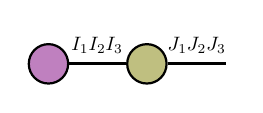
\begin{tikzpicture}[baseline=-0.5ex]
    \tikzset{tensor/.style = {minimum size = 0.5cm,shape = circle,thick,draw=black,inner sep = 0pt}, edge/.style = {thick,line width=.4mm},every loop/.style={}}
    \def\x{0}
    \def\y{0}
     \node[tensor,fill=green!50!red!50!white] (B) at (\x+1,\y) {$\Ab$};
    \node[tensor,fill=blue!50!red!50!white] (a) at (\x-0.25,\y) {$\vb$};
    \draw[edge] (B) -- (\x,\y) node [midway,above] {\scalebox{0.7}{\dimcolor{$I_1I_2I_3$}}};
    \draw[edge] (B) -- (\x+2,\y) node [midway,above] {\scalebox{0.7}{\dimcolor{$J_1J_2J_3$}}};
\end{tikzpicture}
=
\begin{tikzpicture}[baseline=\baseline]
    \tikzset{tensor/.style = {minimum size = 0.5cm,shape = circle,thick,draw=black,inner sep = 0pt}, edge/.style   = {thick,line width=.4mm},every loop/.style={}}
    \def\y{0}
    \def\x{0}
    \node[tensor,fill=red!30!white] (D) at (\x-1.5,\y){$\At_1$};
    \node[tensor,fill=red!50!white] (A) at (\x,\y){$\At_2$};
  \node[tensor,fill=blue!50!white] (B) at (\x+1.5,\y){$\At_3$};
    \draw[edge](A) -- (\x,\y-0.7)node [midway,left] {\edgelabel{$I_2$}};
    \draw[edge](B) -- (\x+1.5,\y-0.7)node [midway,left] {\edgelabel{$I_3$}};
     \draw[edge](D) -- (\x-1.5,\y-0.7)node [midway,left] {\edgelabel{$I_1$}};
    \draw[edge](D) -- (A) node [midway,above] {\edgelabel{$R_1$}};
    \draw[edge](A) -- (B) node [midway,above] {\edgelabel{$R_2$}};
    \draw[edge](A) -- (\x,\y+0.7)node [midway,left] {\edgelabel{$J_2$}};
    \draw[edge](B) -- (\x+1.5,\y+0.7)node [midway,left] {\edgelabel{$J_3$}};
    \draw[edge](D) -- (\x-1.5,\y+0.7)node [midway,left] {\edgelabel{$J_1$}};
    \node[tensor,fill=red!70!blue!40!white] (G1) at (\x-1.5,\y-0.9){$\Gt_1$};
    \node[tensor,fill=red!30!blue!30!white] (G2) at (\x,\y-0.9){$\Gt_2$};
  \node[tensor,fill=red!50!blue!50!white] (G3) at (\x+1.5,\y-0.9){$\Gt_3$};
  \draw[edge] (G1) -- (G2) node [midway,above] {\edgelabel{$S_1$}};
    \draw[edge] (G2) -- (G3) node [midway,above] {\edgelabel{$S_2$}};
\end{tikzpicture}
=~
\begin{tikzpicture}[baseline=\baseline]
    \tikzset{tensor/.style = {minimum size = 0.5cm,shape = circle,thick,draw=black,inner sep = 0pt}, edge/.style   = {thick,line width=.4mm},every loop/.style={}}
    \def\y{0}
    \def\x{0}
    \node[tensor,fill=cyan] (H1) at (\x-1.5,\y){$\Ht_1$};
    \node[tensor,fill=cyan!50!] (H2) at (\x,\y){$\Ht_2$};
   \node[tensor,fill=cyan!20!] (H3) at (\x+1.5,\y){$\Ht_3$};
   \draw[edge] (H1) -- (H2) node [midway,above]{\edgelabel{$R_1S_1$}};
    \draw[edge] (H2) -- (H3) node [midway,above]{\edgelabel{$R_2S_2$}};
    \draw[edge](H1) -- (\x-1.5,\y-0.7) node [midway, left]{\edgelabel{$J_1$}};
    \draw[edge](H2) -- (\x,\y-0.7)node [midway, left]{\edgelabel{$J_2$}};
    \draw[edge](H3) -- (\x+1.5,\y-0.7)node [midway, left]{\edgelabel{$J_3$}};
\end{tikzpicture}.
\end{align}
最后一个等式中，每一对核心张量 $\At_i,\Gt_i$ 被合并为核心 $\Ht_i$~（$i = 1,2,3$），由此得到秩为 $(R_1 S_1, R_2 S_2)$ 的 TT 向量。更一般地，对于 $N$ 阶张量，若 $I_1 = \cdots = I_N = I$，$J_1 = \cdots = J_N = J$，$R_1 = \cdots = R_{N-1} = R$，且 $S_1 = \cdots = S_{N-1} = S$，则矩阵-向量乘积的总计算复杂度为 $\mathcal{O}(N R^2 S^2 I J)$。

上面的矩阵-向量乘积已经表明，在 TT 格式下进行运算会使 TT 秩增大。基础线性代数运算也是如此，
例如求和与张量的逐元素乘积。所得张量仍是 TT 格式，但秩通常因这些运算而增长~\citep{oseledets2010approximation}。这些运算及其对 TT 秩的影响汇总于表~\ref{tab:tt-operations}~\citep{novikov2014putting}。
\begin{table}
\centering
\begin{tabular}{lll}
\toprule
\textsc{运算} & \textsc{输出秩} & \textsc{复杂度} \\
\midrule
$\Ct = \At \cdot \text{const}$ & $R(\Ct) = R(\At)$ & $\mathcal{O}(d\,R(\At))$ \\
$\Ct = \At + \text{const}$ & $R(\Ct) \leq R(\At) + 1$ & $\mathcal{O}(nd\,R(\At)^2)$ \\
$\Ct = \At + \Bt$ & $R(\Ct) \leq R(\At) + R(\Bt)$ & $\mathcal{O}(nd\,R(\Ct)^2)$ \\
$\Ct = \At \krao \Bt$ & $R(\Ct) \leq R(\At)\,R(\Bt)$ & $\mathcal{O}(nd\,R(\At)^2\,R(\Bt)^2)$ \\
$\mathrm{sum} \At$ & -- & $\mathcal{O}(nd\,R(\At)^2)$ \\
$\norm{\At}_F$ & -- & $\mathcal{O}(nd\,R(\mathbf{A})^3)$ \\
\bottomrule
\end{tabular}
\caption{ TT 格式张量上的高效运算~（表格取自~\citep{novikov2014putting}。）}
\label{tab:tt-operations}
\end{table}
表中 $R$ 指最大的 TT 秩，即 $R(\At) = \max_{i=0,\dots,N} R_i$，$n$ 为张量的阶，$d$ 为其最大维数。

需要时，可以用 TT 舍入（TT-rounding）算法~\citep{oseledets2010approximation} 来降低秩~（以一定的近似误差为代价）。

\paragraph{TT 舍入} 如前所述，TT 格式下的张量运算，例如加法或乘法，一般会使 TT 秩增大。为了在保持精度的同时避免秩不受控制地增长，就必须进行秩缩减。这可以通过施加一个 \emph{TT 舍入}流程实现：给定一个 $N$ 阶 TT 张量，其秩为 $R^\prime_k$（$k\in[N-1]$），目标是求出一个 TT 秩 $R_k$ 更低而质量良好的近似。为此，一种朴素而低效的做法是重构整个张量，再执行 TT-SVD，得到秩为 $(R_1,\cdots,R_{N-1})$ 的 TT 近似。事实上，无需重构整个张量就能完成此事！我们将说明，下面这一流程与对整个张量执行 TT-SVD 完全等价。

首先对 TT 核心张量依次做 QR 分解，按自左向右（或自右向左）的扫描完成正交化。随后对每个核心张量施以截断，也就是用截断 SVD 按给定的秩 $R_k$ 舍弃奇异值。被截断的因子再重新分配到相邻的 TT 核心张量中，于是得到一个秩更小、且近似误差受到控制的新 TT 表示。作为示例，考虑一个以 TT 格式给出、秩为 $R^\prime_k$ 的四阶张量。第一步，我们自右向左执行 QR 分解：
\begin{align*}
&\begin{tikzpicture}[baseline=\baseline]
    \tikzset{tensor/.style = {minimum size = 0.5cm,shape = circle,thick,draw=black,inner sep = 0pt}, edge/.style   = {thick,line width=.4mm},every loop/.style={}}
    \def\y{0}
    \def\x{0}
    \node[tensor,fill=cyan] (G1) at (\x-3,\y){$\Gt_1$};
    \node[tensor,fill=cyan!60!] (G2) at (\x-2,\y){$\Gt_2$};
    \node[tensor,fill=cyan!40!] (G3) at (\x-1,\y){$\Gt_3$};
   \node[tensor,fill=cyan!20!] (G4) at (\x,\y){$\Gt_4$};
   \draw[edge] (G1) -- (G2) node [midway,above]{\edgelabel{$R^\prime_1$}};
    \draw[edge] (G2) -- (G3) node [midway,above]{\edgelabel{$R^\prime_2$}};
    \draw[edge] (G3) -- (G4) node [midway,above]{\edgelabel{$R^\prime_3$}};
    \draw[edge](G1) -- (\x-3,\y-0.7) node [midway, left]{\edgelabel{$d_1$}};
    \draw[edge](G2) -- (\x-2,\y-0.7)node [midway, left]{\edgelabel{$d_2$}};
    \draw[edge](G3) -- (\x-1,\y-0.7)node [midway, left]{\edgelabel{$d_3$}};
    \draw[edge](G4) -- (\x,\y-0.7)node [midway, left]{\edgelabel{$d_4$}};
    \node[draw=none] at (\x+3.5,\y){$\underrightarrow{\text{QR decomposition from right to left}}$};
\end{tikzpicture}
\begin{tikzpicture}[baseline=\baseline]
    \tikzset{tensor/.style = {minimum size = 0.5cm,shape = circle,thick,draw=black,inner sep = 0pt}, edge/.style = {thick,line width=.4mm},every loop/.style={}}
    \def\y{0}
    \def\x{0}
        \node[tensor,fill=cyan] (G1) at (\x-3,\y){$\Gt_1$};
    \node[tensor,fill=cyan!60!] (G2) at (\x-2,\y){$\Gt_2$};
    \node[tensor,fill=cyan!40!] (G3) at (\x-1,\y){$\Gt_3$};
    \node[tensor, path picture={
    \fill[fill=cyan!20!](path picture bounding box.south west)
    -- 
    (path picture bounding box.north east) --
    (path picture bounding box.north west) -- cycle;}, shift={(\x+1,\y)}] (G4) {$\Qt_4$};
    \node[tensor,fill=cyan!20!] (R4) at (\x,\y){$\Rb_4$};
   \draw[edge] (G1) -- (G2) node [midway,above]{\edgelabel{$R^\prime_1$}};
    \draw[edge] (G2) -- (G3) node [midway,above]{\edgelabel{$R^\prime_2$}};
    \draw[edge] (G3) -- (R4) node [midway,above]{\edgelabel{$R^\prime_3$}};
    \draw[edge] (R4) -- (G4) node [midway,above]{\edgelabel{$R^\prime_3$}};
    \draw[edge](G1) -- (\x-3,\y-0.7) node [midway, left]{\edgelabel{$d_1$}};
    \draw[edge](G2) -- (\x-2,\y-0.7)node [midway, left]{\edgelabel{$d_2$}};
    \draw[edge](G3) -- (\x-1,\y-0.7)node [midway, left]{\edgelabel{$d_3$}};
    \draw[edge](G4) -- (\x+1,\y-0.7)node [midway,left] {\scalebox{0.7}{\dimcolor{$d_4$}}};
    \node[draw=none] at (\x-0.5,\y+0.7){$\overbrace{\hspace{1cm}}^{\text{merge \& apply QR}}$};
    \end{tikzpicture}\\
&\begin{tikzpicture}[baseline=\baseline]
    \tikzset{tensor/.style = {minimum size = 0.5cm,shape = circle,thick,draw=black,inner sep = 0pt}, edge/.style = {thick,line width=.4mm},every loop/.style={}}
    \def\y{0}
    \def\x{0}
        \node[tensor,fill=cyan] (G1) at (\x-3,\y){$\Gt_1$};
    \node[tensor,fill=cyan!60!] (G2) at (\x-2,\y){$\Gt_2$};
    \node[tensor, path picture={
    \fill[fill=cyan!40!](path picture bounding box.south west)
    -- 
    (path picture bounding box.north east) --
    (path picture bounding box.north west) -- cycle;}, shift={(\x,\y)}] (G3) {$\Qt_3$};
    \node[tensor, path picture={
    \fill[fill=cyan!20!](path picture bounding box.south west)
    -- 
    (path picture bounding box.north east) --
    (path picture bounding box.north west) -- cycle;}, shift={(\x+1,\y)}] (G4) {$\Qt_4$};
    \node[tensor,fill=cyan!40!] (R3) at (\x-1,\y){$\Rb_3$};
   \draw[edge] (G1) -- (G2) node [midway,above]{\edgelabel{$R^\prime_1$}};
    \draw[edge] (G2) -- (R3) node [midway,above]{\edgelabel{$R^\prime_2$}};
    \draw[edge] (R3) -- (G3) node [midway,above]{\edgelabel{$R^\prime_3$}};
    \draw[edge] (G3) -- (G4) node [midway,above]{\edgelabel{$R^\prime_3$}};
    \draw[edge](G1) -- (\x-3,\y-0.7) node [midway, left]{\edgelabel{$d_1$}};
    \draw[edge](G2) -- (\x-2,\y-0.7)node [midway, left]{\edgelabel{$d_2$}};
    \draw[edge](G3) -- (\x,\y-0.7)node [midway, left]{\edgelabel{$d_3$}};
    \draw[edge](G4) -- (\x+1,\y-0.7)node [midway,left] {\scalebox{0.7}{\dimcolor{$d_4$}}};
    \node[draw=none] at (\x-1.5,\y+0.7){$\overbrace{\hspace{1cm}}^{\text{merge \& apply QR}}$};
    \node[draw=none] at (\x+2,\y){$\cdots$};
    \end{tikzpicture}
\begin{tikzpicture}[baseline=\baseline]
    \tikzset{tensor/.style = {minimum size = 0.5cm,shape = circle,thick,draw=black,inner sep = 0pt}, edge/.style = {thick,line width=.4mm},every loop/.style={}}
    \def\y{0}
    \def\x{0}
    \node[tensor,fill=cyan] (G1) at (\x-3,\y){$\Tilde{\Gt_1}$};
    \node[tensor, path picture={
    \fill[fill=cyan!60!](path picture bounding box.south west)
    -- 
    (path picture bounding box.north east) --
    (path picture bounding box.north west) -- cycle;}, shift={(\x-2,\y)}] (G2) {$\Qt_2$};
    \node[tensor, path picture={
    \fill[fill=cyan!40!](path picture bounding box.south west)
    -- 
    (path picture bounding box.north east) --
    (path picture bounding box.north west) -- cycle;}, shift={(\x-1,\y)}] (G3) {$\Qt_3$};
    \node[tensor, path picture={
    \fill[fill=cyan!20!](path picture bounding box.south west)
    -- 
    (path picture bounding box.north east) --
    (path picture bounding box.north west) -- cycle;}, shift={(\x,\y)}] (G4) {$\Qt_4$};
   \draw[edge] (G1) -- (G2) node [midway,above]{\edgelabel{$R^\prime_1$}};
      \draw[edge] (G2) -- (G3) node [midway,above]{\edgelabel{$R^\prime_2$}};
    \draw[edge] (G3) -- (G4) node [midway,above]{\edgelabel{$R^\prime_3$}};
    \draw[edge](G1) -- (\x-3,\y-0.7) node [midway, left]{\edgelabel{$d_1$}};
    \draw[edge](G2) -- (\x-2,\y-0.7)node [midway, left]{\edgelabel{$d_2$}};
    \draw[edge](G3) -- (\x-1,\y-0.7)node [midway, left]{\edgelabel{$d_3$}};
    \draw[edge](G4) -- (\x,\y-0.7)node [midway,left] {\scalebox{0.7}{\dimcolor{$d_4$}}};
    \end{tikzpicture}.
\end{align*}
随后自左向右继续施加截断 SVD：
\begin{align*}
&\begin{tikzpicture}[baseline=\baseline]
    \tikzset{tensor/.style = {minimum size = 0.5cm,shape = circle,thick,draw=black,inner sep = 0pt}, edge/.style = {thick,line width=.4mm},every loop/.style={}}
    \def\x{0}
    \def\y{0}
    \node[tensor,fill=cyan] (G1) at (\x-3,\y){$\Tilde{\Gt_1}$};
    \node[tensor, path picture={
    \fill[fill=cyan!60!](path picture bounding box.south west)
    -- 
    (path picture bounding box.north east) --
    (path picture bounding box.north west) -- cycle;}, shift={(\x-2,\y)}] (G2) {$\Qt_2$};
    \node[tensor, path picture={
    \fill[fill=cyan!40!](path picture bounding box.south west)
    -- 
    (path picture bounding box.north east) --
    (path picture bounding box.north west) -- cycle;}, shift={(\x-1,\y)}] (G3) {$\Qt_3$};
    \node[tensor, path picture={
    \fill[fill=cyan!20!](path picture bounding box.south west)
    -- 
    (path picture bounding box.north east) --
    (path picture bounding box.north west) -- cycle;}, shift={(\x,\y)}] (G4) {$\Qt_4$};
   \draw[edge] (G1) -- (G2) node [midway,above]{\edgelabel{$R^\prime_1$}};
      \draw[edge] (G2) -- (G3) node [midway,above]{\edgelabel{$R^\prime_2$}};
    \draw[edge] (G3) -- (G4) node [midway,above]{\edgelabel{$R^\prime_3$}};
    \draw[edge](G1) -- (\x-3,\y-0.7) node [midway, left]{\edgelabel{$d_1$}};
    \draw[edge](G2) -- (\x-2,\y-0.7)node [midway, left]{\edgelabel{$d_2$}};
    \draw[edge](G3) -- (\x-1,\y-0.7)node [midway, left]{\edgelabel{$d_3$}};
    \draw[edge](G4) -- (\x,\y-0.7)node [midway,left] {\scalebox{0.7}{\dimcolor{$d_4$}}};
    \node[draw=none] at (\x+3.25,\y){$\underrightarrow{\text{rank-$R_1$ truncated SVD of $\tilde \Gt_1$}}$};
    \end{tikzpicture}
\begin{tikzpicture}[baseline=\baseline]
    \tikzset{tensor/.style = {minimum size = 0.5cm,shape = circle,thick,draw=black,inner sep = 0pt}, edge/.style = {thick,line width=.4mm},every loop/.style={}}
    \def\y{0}
    \def\x{0}
     \node[tensor, path picture={
    \fill[fill=cyan](path picture bounding box.south east)
    -- 
    (path picture bounding box.north west) --
    (path picture bounding box.north east) -- cycle;}, shift={(\x-3,\y)}] (U1) {$\Gt_1$};
    \node[tensor,fill=cyan] (sigma) at (\x-2,\y){{}};
    \draw[edge=0.5] (sigma.south west) -- (sigma.north        east);
    \node[tensor, path picture={
    \fill[fill=cyan](path picture bounding box.south west)
    -- 
    (path picture bounding box.north east) --
    (path picture bounding box.north west) -- cycle;}, shift={(\x-1,\y)}] (V1) {$\Vb_1$};
    \node[tensor, path picture={
    \fill[fill=cyan!60!](path picture bounding box.south west)
    -- 
    (path picture bounding box.north east) --
    (path picture bounding box.north west) -- cycle;}, shift={(\x,\y)}] (G2) {$\Qt_2$};
    \node[tensor, path picture={
    \fill[fill=cyan!40!](path picture bounding box.south west)
    -- 
    (path picture bounding box.north east) --
    (path picture bounding box.north west) -- cycle;}, shift={(\x+1,\y)}] (G3) {$\Qt_3$};
    \node[tensor, path picture={
    \fill[fill=cyan!20!](path picture bounding box.south west)
    -- 
    (path picture bounding box.north east) --
    (path picture bounding box.north west) -- cycle;}, shift={(\x+2,\y)}] (G4) {$\Qt_4$};
   \draw[edge] (U1) -- (sigma) node [midway,above]{\edgelabel{$R_1$}};
      \draw[edge] (sigma) -- (V1) node [midway,above]{\edgelabel{$R_1$}};
    \draw[edge] (V1) -- (G2) node [midway,above]{\edgelabel{$R_1$}};
    \draw[edge] (G2) -- (G3) node [midway,above]{\edgelabel{$R^\prime_2$}};
    \draw[edge] (G3) -- (G4) node [midway,above]{\edgelabel{$R^\prime_3$}};
    \draw[edge](U1) -- (\x-3,\y-0.7) node [midway, left]{\edgelabel{$d_1$}};
    \draw[edge](G2) -- (\x,\y-0.7)node [midway, left]{\edgelabel{$d_2$}};
    \draw[edge](G3) -- (\x+1,\y-0.7)node [midway, left]{\edgelabel{$d_3$}};
    \draw[edge](G4) -- (\x+2,\y-0.7)node [midway,left] {\scalebox{0.7}{\dimcolor{$d_4$}}};
    \node[draw=none] at (\x-1,\y+0.7){$\overbrace{\hspace{2cm}}^{\text{merge \& apply rank-$R_2$ SVD}}$};
    \end{tikzpicture}\\
&\begin{tikzpicture}[baseline=\baseline]
    \tikzset{tensor/.style = {minimum size = 0.5cm,shape = circle,thick,draw=black,inner sep = 0pt}, edge/.style = {thick,line width=.4mm},every loop/.style={}}
    \def\y{0}
    \def\x{0}
     \node[tensor, path picture={
    \fill[fill=cyan](path picture bounding box.south east)
    -- 
    (path picture bounding box.north west) --
    (path picture bounding box.north east) -- cycle;}, shift={(\x-3,\y)}] (U1) {$\Gt_1$};
    \node[tensor, path picture={
    \fill[fill=cyan!60!](path picture bounding box.south east)
    -- 
    (path picture bounding box.north west) --
    (path picture bounding box.north east) -- cycle;}, shift={(\x-2,\y)}] (G2) {$\Gt_2$};
    \node[tensor,fill=cyan!60!] (sigma) at (\x-1,\y){{}};
    \draw[edge=0.5] (sigma.south west) -- (sigma.north        east);
    \node[tensor, path picture={
    \fill[fill=cyan!60!](path picture bounding box.south west)
    -- 
    (path picture bounding box.north east) --
    (path picture bounding box.north west) -- cycle;}, shift={(\x,\y)}] (V2) {$\Vb_2$};
    \node[tensor, path picture={
    \fill[fill=cyan!40!](path picture bounding box.south west)
    -- 
    (path picture bounding box.north east) --
    (path picture bounding box.north west) -- cycle;}, shift={(\x+1,\y)}] (G3) {$\Qt_3$};
    \node[tensor, path picture={
    \fill[fill=cyan!20!](path picture bounding box.south west)
    -- 
    (path picture bounding box.north east) --
    (path picture bounding box.north west) -- cycle;}, shift={(\x+2,\y)}] (G4) {$\Qt_4$};
   \draw[edge] (U1) -- (G2) node [midway,above]{\edgelabel{$R_1$}};
      \draw[edge] (G2) -- (sigma) node [midway,above]{\edgelabel{$R_2$}};
    \draw[edge] (sigma) -- (V2) node [midway,above]{\edgelabel{$R_2$}};
    \draw[edge] (V2) -- (G3) node [midway,above]{\edgelabel{$R^\prime_2$}};
    \draw[edge] (G3) -- (G4) node [midway,above]{\edgelabel{$R^\prime_3$}};
    \draw[edge](U1) -- (\x-3,\y-0.7) node [midway, left]{\edgelabel{$d_1$}};
    \draw[edge](G2) -- (\x-2,\y-0.7)node [midway, left]{\edgelabel{$d_2$}};
    \draw[edge](G3) -- (\x+1,\y-0.7)node [midway, left]{\edgelabel{$d_3$}};
    \draw[edge](G4) -- (\x+2,\y-0.7)node [midway,left] {\scalebox{0.7}{\dimcolor{$d_4$}}};
    \node[draw=none] at (\x,\y+0.7){$\overbrace{\hspace{2cm}}^{\text{merge \& apply rank-$R_3$ SVD}}$};
    \node[draw=none] at (\x+3,\y){$\longrightarrow$};
    \end{tikzpicture}
\begin{tikzpicture}[baseline=\baseline]
    \tikzset{tensor/.style = {minimum size = 0.5cm,shape = circle,thick,draw=black,inner sep = 0pt}, edge/.style = {thick,line width=.4mm},every loop/.style={}}
    \def\y{0}
    \def\x{0}
     \node[tensor, path picture={
    \fill[fill=cyan](path picture bounding box.south east)
    -- 
    (path picture bounding box.north west) --
    (path picture bounding box.north east) -- cycle;}, shift={(\x-3,\y)}] (U1) {$\Gt_1$};
    \node[tensor, path picture={
    \fill[fill=cyan!60!](path picture bounding box.south east)
    -- 
    (path picture bounding box.north west) --
    (path picture bounding box.north east) -- cycle;}, shift={(\x-2,\y)}] (G2) {$\Gt_2$};
    \node[tensor, path picture={
    \fill[fill=cyan!40!](path picture bounding box.south east)
    -- 
    (path picture bounding box.north west) --
    (path picture bounding box.north east) -- cycle;}, shift={(\x-1,\y)}] (G3) {$\Gt_3$};
    \node[tensor,fill=cyan!40!] (sigma) at (\x,\y){{}};
    \draw[edge=0.5] (sigma.south west) -- (sigma.north        east);
    \node[tensor, path picture={
    \fill[fill=cyan!40!](path picture bounding box.south west)
    -- 
    (path picture bounding box.north east) --
    (path picture bounding box.north west) -- cycle;}, shift={(\x+1,\y)}] (V3) {$\Vb_3$};
    \node[tensor, path picture={
    \fill[fill=cyan!20!](path picture bounding box.south west)
    -- 
    (path picture bounding box.north east) --
    (path picture bounding box.north west) -- cycle;}, shift={(\x+2,\y)}] (G4) {$\Qt_4$};
   \draw[edge] (U1) -- (G2) node [midway,above]{\edgelabel{$R_1$}};
      \draw[edge] (G2) -- (G3) node [midway,above]{\edgelabel{$R_2$}};
    \draw[edge] (G3) -- (sigma) node [midway,above]{\edgelabel{$R_3$}};
    \draw[edge] (sigma) -- (V3) node [midway,above]{\edgelabel{$R_3$}};
    \draw[edge] (V3) -- (G4) node [midway,above]{\edgelabel{$R^\prime_3$}};
    \draw[edge](U1) -- (\x-3,\y-0.7) node [midway, left]{\edgelabel{$d_1$}};
    \draw[edge](G2) -- (\x-2,\y-0.7)node [midway, left]{\edgelabel{$d_2$}};
    \draw[edge](G3) -- (\x-1,\y-0.7)node [midway, left]{\edgelabel{$d_3$}};
    \draw[edge](G4) -- (\x+2,\y-0.7)node [midway,left] {\scalebox{0.7}{\dimcolor{$d_4$}}};
    \node[draw=none] at (\x+1,\y+0.7){$\overbrace{\hspace{2cm}}^{\text{merge}}$};
    \node[draw=none] at (\x+3,\y){$\longrightarrow$};
    \end{tikzpicture}\\
&\begin{tikzpicture}[baseline=\baseline]
    \tikzset{tensor/.style = {minimum size = 0.5cm,shape = circle,thick,draw=black,inner sep = 0pt}, edge/.style = {thick,line width=.4mm},every loop/.style={}}
    \def\y{0}
    \def\x{0}
     \node[tensor, path picture={
    \fill[fill=cyan](path picture bounding box.south east)
    -- 
    (path picture bounding box.north west) --
    (path picture bounding box.north east) -- cycle;}, shift={(\x-3,\y)}] (U1) {$\Gt_1$};
    \node[tensor, path picture={
    \fill[fill=cyan!60!](path picture bounding box.south east)
    -- 
    (path picture bounding box.north west) --
    (path picture bounding box.north east) -- cycle;}, shift={(\x-2,\y)}] (G2) {$\Gt_2$};
    \node[tensor, path picture={
    \fill[fill=cyan!40!](path picture bounding box.south east)
    -- 
    (path picture bounding box.north west) --
    (path picture bounding box.north east) -- cycle;}, shift={(\x-1,\y)}] (G3) {$\Gt_3$};
    \node[tensor,fill=cyan!20!] (G4) at (\x,\y){$\Gt_4$};
   \draw[edge] (U1) -- (G2) node [midway,above]{\edgelabel{$R_1$}};
      \draw[edge] (G2) -- (G3) node [midway,above]{\edgelabel{$R_2$}};
    \draw[edge] (G3) -- (G4) node [midway,above]{\edgelabel{$R_3$}};
    \draw[edge](U1) -- (\x-3,\y-0.7) node [midway, left]{\edgelabel{$d_1$}};
    \draw[edge](G2) -- (\x-2,\y-0.7)node [midway, left]{\edgelabel{$d_2$}};
    \draw[edge](G3) -- (\x-1,\y-0.7)node [midway, left]{\edgelabel{$d_3$}};
    \draw[edge](G4) -- (\x,\y-0.7)node [midway,left] {\scalebox{0.7}{\dimcolor{$d_4$}}};
    \end{tikzpicture},   
\end{align*}
